\documentclass[12pt,a4paper,ngerman,english]{report}
\usepackage[utf8]{inputenc}
\usepackage[german]{babel}
\usepackage[draft]{todonotes} 
\usepackage{pdfpages}
\usepackage{pdflscape}
\usepackage{rotating}
\usepackage{epstopdf}
\usepackage{cite}
\usepackage{graphicx}
\usepackage{gensymb}
\usepackage{amsmath}
\usepackage{amssymb}
\usepackage{float}
\usepackage{fancyhdr}
\usepackage{textcomp}
\usepackage[numbers]{natbib}
\usepackage{varioref}
\usepackage{hyperref}
\usepackage[ngerman]{cleveref}
\usepackage{listings}

\usepackage[a4paper, top=30mm, left=30mm, right=30mm, bottom=30mm,headsep=10mm, footskip=12mm]{geometry}
\parindent0pt

%\usepackage[sorting=nyt, backend=biber, style=alphabetic]{biblatex}
%\addbibresource{mybib.bib}

\usepackage[onehalfspacing]{setspace}

\graphicspath{graphics}

\newcommand\tab[1][1cm]{\hspace*{#1}}

\pagestyle{fancy} %eigener Seitenstil
\fancyhf{} %alle Kopf- und Fußzeilenfelder bereinigen
\fancyhead[L]{\small{\leftmark}}

\renewcommand{\headrulewidth}{0.1pt} %obere Trennlinie
\fancyfoot[C]{\thepage} %Seitennummer
\setlength{\headheight}{13.6pt}

%\lstset{language=C++, basicstyle=\ttfamily\footnotesize, showstringspaces=false} %C++ code formatierung
\lstset{language=C++,
	basicstyle=\ttfamily\footnotesize,
	breaklines=true,
	%	literate={\ \ }{{\ }}1, 
	showstringspaces=false,
	keywordstyle=\color{blue}\ttfamily,
	stringstyle=\color{red}\ttfamily,
	commentstyle=\color{green}\ttfamily,
	morecomment=[l][\color{magenta}]{\#}
}

\newenvironment{abstractpage}
{\cleardoublepage\vspace*{\fill}\thispagestyle{empty}}
{\vfill\cleardoublepage}
\newenvironment{abstrac}[1]
{\bigskip\selectlanguage{#1}%
	\begin{center}\bfseries\abstractname\end{center}}
{\par\bigskip}

\begin{document}

%Titlepage
\begin{titlepage}
\begin{center}	
	\Huge{PirateBayTours}
	
	\line(1,0){400} \\
	\textsc{\Large Projekt im Modul Verteilte Informationsysteme WS2016/17}\\
	[8cm]

	{\Large\itshape Jesko Appelfeller\footnote{Matrikelnr.: 916832} \par Frederik Broer\footnote{Matrikelnr.: 789617} \par Jonas Droste\footnote{Matrikelnr.: 897553} \par Robin Naundorf\footnote{Matrikelnr.: 636612} \par }
	\vfill

	\large{betreut durch\par
		Prof. Dr.-Ing. Thomas Christian \textsc{Weik}}

	\vfill
	{\large \today\par}

\end{center}
\end{titlepage}


% Abstracts
\newpage
\begin{abstractpage}
	\begin{abstrac}{ngerman}
    Im Modul ``Verteilte Informationssysteme'' wurde die Aufgabe gestellt, eine Software zur Buchung von Tickets für Bootstouren zu entwickeln. Hierbei bestand die Schwierigkeit, dass die Vertriebsagenten nur vor Beginn und nach Ende des Ticketverkaufs Internetzugang benötigen sollten. Es war also eine Lösung zu entwickeln, die es ermöglicht sowohl Angaben über Touren und Boote als auch die Buchung von Tickets offline vorzuhalten und zu den gegebenen Zeitpunkten mit Internetzugang zu synchronisieren. Insbesondere interessant war die Replikation der offline-Buchungen zurück zum Server, da hier Potential für Konflikte mit den Buchungen anderer Agenten bestand. Dieses Dokument beschreibt eine solche Lösung basierend auf einem PostgreSQL-Server mit einem RESTful Python-API mittels des Django-Frameworks als Backend, sowie einem Client der mittels Java und SQLite implementiert wurde.
	\end{abstrac}
	\begin{abstrac}{english}
    In the class ``Distributed Information Systems'' a task was set for the students to implement an application for booking tickets for boat tours. As an added challenge, the sales agents would only have internet access before starting and after finishing their sales. Therefore, a solution was to be developed that would enable both the offline storage of boats and tours and the offline booking of tickets as well as the synchronisation of those bookings once internet access had been established. The latter area was of special interest, as there were potential conflicts with bookings from other agents to resolve. This document describes one such solution based on a PostgreSQL-server with a RESTful Python API using the Django framework, as well as a client implemented in Java and using SQLite. 
	\end{abstrac}
\end{abstractpage}



\newpage
\tableofcontents

\chapter{Motivation und Anforderungen}
Im Rahmen des Moduls 'Verteilte Informationssysteme' an der Fachhochschule Münster wird ein Semester begleitendes Datenbank Projekt durchgeführt. Ziel des Projektes ist es, ein Buchungssystem für Bootstouren zu implementieren. Die Firma Pirate-Bay-Tours beschäftigt mehrere Vertriebsmitarbeiter, die an Touristen Hotspots Tickets für Boots"-touren vertreiben. Für diese Mitarbeiter soll ein neues Buchungssystem implementiert werden.\\
Wichtigstes Funktionsmerkmal des Systems ist die Offline-Fähigkeit. Das heißt, auch wenn der Mitarbeiter keine Verbindung zum zentralen Buchungsserver hat, muss die Buchung von Touren möglich sein. Dazu soll eine Replikationslogik entwickelt werden, die offline getätigte Buchungen bei verfügbarer Online-Verbindung mit dem Server synchronisiert. Weiterhin soll ein Quotensystem entwickelt werden, mit dem es möglich ist, verfügbare Tourtickets auf unterschiedliche Agenten zu verteilen. Zusätzlich muss eine Strategie entwickelt werden, wie mit Überbuchungen umgegangen werden soll.

\chapter{Lösungskonzept}
\section{Architektur}

Das Projekt PirateBayTours besteht aus einer Client-Server-Architektur. Die Agenten arbeiten mit einem Client auf Java-Basis. Eine Synchronisierung mit dem Server erfolgt mittels HTTP-Rest aufrufen. Der Server basiert auf Python 3\footnote{https://www.python.org} und dem Django Web-Framework\footnote{https://www.djangoproject.com} . Für die Implementierung der Rest-API wurde das Paket \textit{django-rest-framework}\footnote{https://www.django-rest-framework.org} verwendet. Für das Load-Balancing der Postgres-Instanzen wurde ein Software-Loadbalancer auf Basis von VMware NSX\footnote{https://www.vmware.com/products/nsx.html} verwendet. Eine schematische Darstellung findet sich in Abbildung \ref{fig:architecture}

\begin{figure}[h]
	\centering
	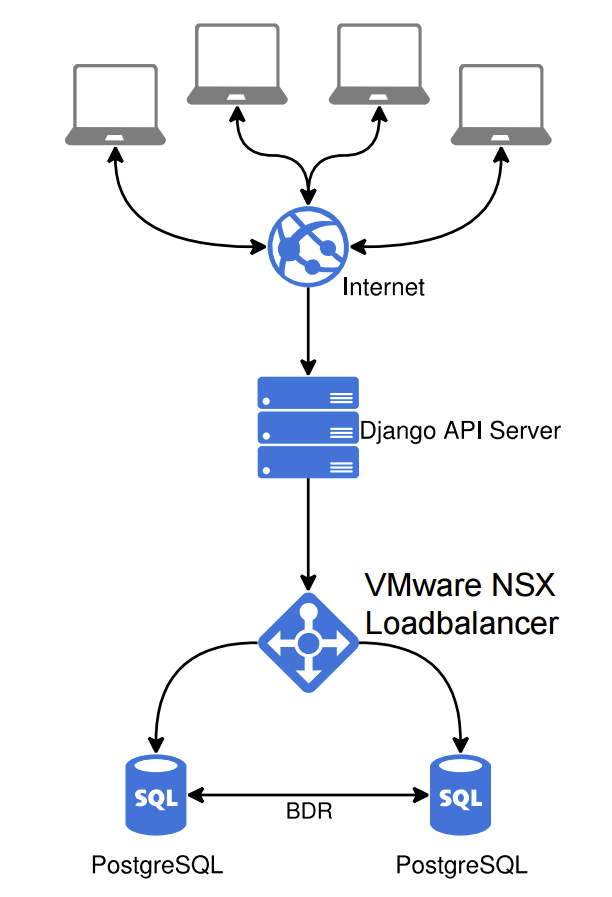
\includegraphics[width=0.6\textwidth]{img/architecture.png}
	\caption{Architektur}
	\label{fig:architecture}
\end{figure}


\section{Backend}
\subsection{Django und Admin Interface}\label{sec:django-und-admin-interface}
Für das Backend wurde Django in der Version 1.10.5 verwendet. Django bietet als Framework unter anderem einen Object-Relational-Mapper (kurz: ORM) der bei der Abstrahierung der Datenbank-Schicht hilft. Django basiert auf dem MVC-Prinzip. Hierdurch ist es möglich in der Modell-Schicht ein Modell zu implementieren, dass dann mittels ORM als Schema in der Datenbank abgelegt wird. Das Implementierte Modell ist in Abbildung \ref{fig:django-modell} zu sehen.

Mit Hilfe des  Django-Rest-Frameworks wird der Zugriff auf das Backend mittels HTTP-Rest-Aufrufen realisiert. Es ist z.B. möglich alle vorhanden Touren über einen HTTP-GET-Aufruf an http://SERVER/api/tours  zu bekommen. Der Server liefert die angeforderten Daten im JSON-Format\footnote{http://www.json.org/} zurück.

Für die Administration der Datenbestände (z.B. Hinzufügen neuer Touren/Schiffe) bietet Django ein integriertes Admin-Backend mit Authentifizierung über Benutzername/Passwort.

\begin{figure}[h]
	\centering
	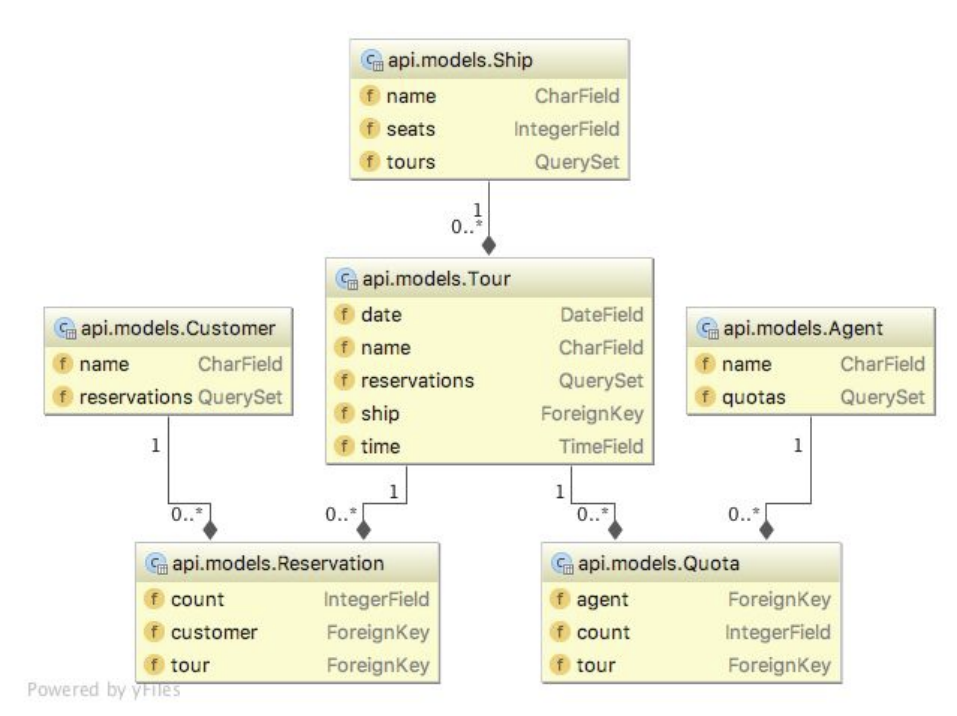
\includegraphics[width=0.6\textwidth]{img/django-modell.png}
	\caption{Django Modell}
	\label{fig:django-modell}
\end{figure}

\subsection{Datenbank}

Die Datenbank für das Projekt PirateBayTours basiert auf PostgreSQL. Die Replizierung der Datenbank serverseitig erfolgt mittels einer angepassten PostgreSQL-Version zur bidirektionalen Replikation \textit{Postgres-BDR} der Firma 2ndQuandrant. Für die Hochverfügbarkeit der Datenbank wurden 2 Server mit Debian-Linux aufgesetzt auf denen jeweils eine Postgres-Datenbank in der BDR-Anpassung von 2ndQuadrant läuft. Diese beiden Datenbanken synchronisieren sich ständig und sind beide sowohl lesend als auch schreibend benutzbar (sogenannte Multi-Master-Replikation).


\subsubsection{Replikation}

Eine vorgefertigte Replikationslösung zwischen SQLite und PostgreSQL gibt es nicht. Daher wird die Replikation in Eigenentwicklung umgesetzt. Für Details siehe \autoref{sec:Replizierung}.

\section{Client}
\subsection{Java Client}
\subsubsection{Implementierungsmodell}
Wir haben uns dazu entschieden den Client in der Programmiersprache Java zu schreiben, dadurch konnte unsere gesamte Gruppe gemeinsam an den Implementierungen für den Client arbeiten, weil Java eine Standardprogrammiersprache ist die jeder aus unserer Gruppe beherrschte. Außerdem ist Java sehr praktikabel für die Implementierung einer graphischen Oberfläche, wie sie für einen benutzerfreundlichen Client nötig ist.\\

\begin{figure}[h]
  \centering
  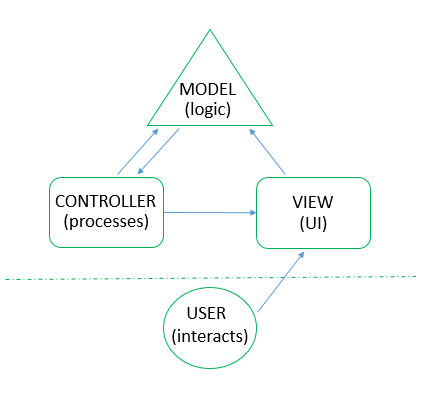
\includegraphics[width=0.6\textwidth]{img/mvc.png}
  \caption{Darstellung des MVC Modells}
  \label{fig:MVC}
\end{figure}

Für die Implementierung haben wir das MVC-Modell („Model-View-Controller“-Modell) verwendet, welches für die Umsetzung unserer Aufgabe sehr geeignet war.\\
Das MVC-Modell teilt die Implementierung in drei unterschiedliche Komponenten ein:	
\begin{itemize}
	\setlength\itemsep{0.1em}
	\item \texttt{das Datenmodell (engl. model),}
	\item \texttt{die Präsentation (engl. view) und}
	\item \texttt{die Programmsteuerung (engl. controller).}
\end{itemize}
Daher benötigen wir drei unterschiedliche Klassen, die in Abbildung \ref{fig:MVC}\footnote{http://docs.sitefinity.com/sf-images/default-source/default-album/mvc.png} dargestellt sind. In der Klasse „model“ wurden die darzustellenden Daten gespeichert, wie beispielsweise der Routenname, in der die ausgewählte Route zwischengespeichert wird. In der Klasse „view“ wurden die benötigten Daten aus dem „model“ dargestellt und die Benutzerinteraktionen entgegengenommen. In der Klasse „controller“ wurde die Steuerung Implementiert, die für die Bearbeitung der Benutzerinteraktionen zuständig ist. Zusätzlich zu diesen drei Klassen des MVC-Modells, haben wir eine Klasse für die API-Zugriffe sowie eine Klasse für Zugriffe auf die SQLite Cache-Datenbank erstellt.
\subsubsection{Struktur}
Nachdem im letzten Kapitel das Implementierungsmodell dargestellt wurde, folgt nun die Beschreibung der Struktur des Clients. Der Client ist wie in Abbildung \ref{fig:Client} dargestellt. Diese sehr simple Darstellung der Oberflächenelemente und die dadurch entstehende  hohe Benutzerfreundlichkeit ist ein großer Vorteil unseres Clients. Die einfache Bedienbarkeit entsteht insbesondere durch die Möglichkeit die Anwendung nur mit der Tastatur zu bedienen. Dadurch können beispielsweise viele Tickets in kürzester Zeit verkauft werden.
\begin{figure}[h]
  \centering
  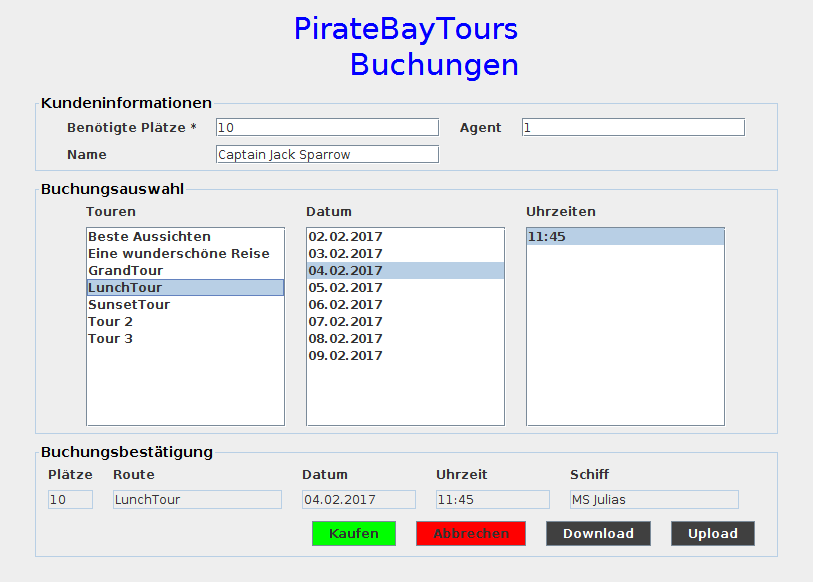
\includegraphics[width=0.94\textwidth]{img/Client.png}
  \caption{Darstellung des Clients}
  \label{fig:Client}
\end{figure}
\newpage
Beim Start der Anwendung müssen zunächst die Daten, also die bisher nicht verkauften Tickets sowie alle anderen notwendigen Daten vom Server geladen werden. Hierfür wird die Schaltfläche „Download“ angeklickt. Anschließend liegen die aktuellen Daten in der lokalen Datenbank und können verwendet und bearbeitet werden. In das Textfeld „Agent“ muss die Personalnummer des jeweiligen Vertriebsmitarbeiters eingetragen werden.\\

Damit Tickets für eine bestimmte Route gebucht werden können, müssen folgende Schritte nacheinander durchgeführt werden.

\begin{enumerate}
\item Die Anzahl der benötigten Tickets sowie der Name des Käufers müssen in die entsprechenden Textfelder eingetragen werden. Anschließend steht im Textfeld „Plätze“ der eingetragene Wert.
\item Nach der Bestätigung mit der „Enter“-Taste werden die Touren angezeigt, für die noch genügend Plätze vorhanden sind.
\item Sobald eine Tour, durch die Selektion einer Zeile, ausgewählt wurde, wird die ausgewählte Route im Textfeld „Route“ angegeben.
\item Nun werden in der Liste „Datum“ alle möglichen Daten angegeben, an denen die Tour gebucht werden kann.
\item Mit der Auswahl eines Datums und der zugehörigen Selektion einer Zeile wird im Textfeld „Datum“ das gewählte Datum angegeben und in der Liste „Uhrzeiten“ werden die möglichen Uhrzeiten für die gewählte Tour sowie Datum angezeigt.
\item Erst mit der Auswahl einer Uhrzeit wird die Schaltfläche "Kaufen" aktiviert womit ein Ticket, bzw. mehrere Tickets gebucht werden können.
\end{enumerate}
Mit der Schaltfläche „Abbrechen“ kann die Buchung jederzeit beendet werden und alle Textfelder, bis auf das Textfeld „Agent“, werden zurückgesetzt. Nachdem der Arbeitstag beendet ist, oder der Vertriebsmitarbeiter zwischenzeitlich eine Internetverbindung aufnehmen kann, können die bisher verkauften Tickets mit dem Server synchronisiert werden. Dafür muss lediglich die Schaltfläche „Upload“ angeklickt werden.\\


\subsection{Lokale Cache DB}
Um offline einsatzfähig zu sein, wurde eine lokale SQLite Datenbank genutzt. Während der Synchronisierung vom Server zum Client wird ein Abbild der Serverdatenbank heruntergeladen und in der lokalen Datenbank gecached. Wir haben uns entschieden eine SQLite Datenbank zu nutzen, da keine zusätzlich Datenbankserver installiert werden müssen und alle notwendigen Ressourcen gut in die Applikation eingebunden werden können. Weiterhin wird SQLite von einer Vielzahl an Programmiersprachen gut unterstützt und bietet eine ressourcensparende Möglichkeit Daten abzulegen. \\

Wie erwähnt, enthält die Datenbank nach einmalige Synchronisation ein komplett Abbild der Server-Datenbank. Das heißt, lokal sind folgende Tabellen verfügbar:
\begin{itemize}
	\setlength\itemsep{0.1em}
	\item \texttt{agents}
	\item \texttt{customers}
	\item \texttt{quotas}
	\item \texttt{ships}
	\item \texttt{tours}
\end{itemize}
Zusätzlich dazu werden zwei lokale Tabellen angelegt.
\begin{itemize}
	\setlength\itemsep{0.1em}
	\item \texttt{offline\_bookings}
	\item \texttt{offline\_customers}
\end{itemize}
Die \texttt{offline\_bookings} Tabelle enthält alle Buchungen, die der Vertriebsmitarbeiter im Offline-Fall tätigt. Werden im Offline-Modus neue Kundenstammdaten angelegt werden diese in der Tabelle \texttt{offline\_customers} gespeichert. Dies ist notwendig, um ID Konflikte bei der Replizierung zu vermeiden. Weiterhin lässt sich so mit wenig Aufwand nachvollziehen welche Buchungen noch nicht repliziert wurden. Da das Serverabbild bei einer Offline-Buchung nicht verändert wird, besteht kein Risiko, dass es zu inkonsistenten Ausgangsdaten kommt und ein Offline-Arbeiten nicht mehr möglich ist.

\section{Replizierung}
\label{sec:Replizierung}

Wie in \autoref{sec:RepliZeit} beschrieben, gibt es zwei Replikationsprozesse. Zum einen lesend vom Server zur lokalen DB, zum anderen schreibend, von der lokalen DB zum Server.

\subsection{Lesende Replizierung}

Der lesende Replikationsvorgang ist trivial. Die Inhalte der Tabellen \texttt{agents, customers, quotas, ships} und \texttt{tours} werden per HTTP bei der Django-API angefragt und von dieser als JSON zurückgegeben. Clientseitig werden diese JSON-Strings geparst und in die lokale DB eingefügt. Vergleiche hierzu Kapitel \ref{sec:django-und-admin-interface}

\subsection{Schreibende Replizierung}
\label{subsec:SchrRepl}

Bei der schreibenden Replizierung sollen die Eintrage der Tabellen \texttt{offline\_customers} und \texttt{offline\_bookings} aus der lokalen Datenbank an die Tabellen \texttt{customers} und \texttt{bookings} der zentralen Datenbank übertragen werden. Dies geschieht, analog zum lesenden Zugriff, durch Umformung der Einträge in JSON-Objekte welche dann mittels HTTP-Requests an die Django-API geschickt werden.\\

Hierbei ergibt sich die Schwierigkeit, dass die Einträge in der lokalen DB automatisch eine ID bekommen haben, die jedoch nur lokal gültig ist. Bei der Übertragung werden neue, dort gültige IDs für jeden Eintrag vergeben. Dies bedeutet jedoch, dass die Verweise aus der \texttt{offline\_bookings} Tabelle auf IDs in der \texttt{offline\_customers} Tabelle serverseitig nicht mehr gültig sind. Vergleiche hierzu Kapitel \ref{sec:django-und-admin-interface}, Abbildung \ref{fig:django-modell}\\

Es müssen also vor dem Upload der Einträge aus der Tabelle \texttt{offline\_bookings} die Verweise auf die lokalen IDs in der Tabelle \texttt{offline\_customers} ersetzt werden durch Verweise auf die zentralen IDs in der Tabelle \texttt{customers}. Diese werden aber vom Server erst vergeben, wenn die Einträge aus der \texttt{offline\_customers} zum Server gesendet werden. Die bereits erwähnte Django-API beantwortet jeden erfolgreichen Schreibzugriff mit dem Versand des erzeugten Eintrags als JSON-Objekt. Diese Objekte enthalten die vom Server vergebene ID die somit direkt in den entsprechenden Datensatz der lokalen \texttt{offline\_customers} eingetragen werden kann.\\

Es werden jedoch nicht die lokalen IDs überschrieben, sondern die zentralen IDs hinzugefügt. Dies ermöglicht es in einem zweiten Schritt für jeden Eintrag der Tabelle \texttt{offline\_bookings} den Verweis von der lokalen auf die zentrale ID anzupassen und den Eintrag dann zum Server zu senden.\\

Nach Abschluss der Replikation werden die Einträge der Tabellen \texttt{offline\_bookings} und \texttt{offline\_customers} nicht mehr benötigt. Beide Tabellen werden gelöscht und neu angelegt, um Duplikate sicher auszuschließen. Der gesamte Vorgang wird in \autoref{fig:ReplSchreibend} graphisch dargestellt.

\begin{figure}[h]
  \centering
  \includegraphics{img/Flowchart_VerSys.png}
  \caption{Ablaufdiagramm schreibende Replikation}
  \label{fig:ReplSchreibend}
\end{figure}

\chapter{Geschäftslogik}
\section{Buchungslogik}
\label{sec:Buchungslogik}

Ein entscheidender Punkt in der Geschäftslodig einer Anwendung wie der piratebaytours ist der Bereich der Buchungslogik. Da die Angenten die meiste Zeit offline arbeiten, muss ein Weg gefunden werden einerseits den Angenten den Spielraum zu geben um auch größeren Gruppen Angebote machen zu können. Andererseits sollten Überbuchungen vermieden werden, da diese zu Verstimmungen bei den Kunden sowie Rück- oder gar Entschädigungszahlungen für das Unternehmen führen.\\

Es müssen also die vorhandenen Plätze auf jedem Schiff und jeder Route auf die Agenten verteilt werden, in solch einer Weise dass das Kontingent dem einzelnen Agenten möglichst reicht. Unser Lösungsansatz besteht darin, Überbuchungen generell nicht zuzulassen. Stattdessen berechnen wir jede Nacht die Kontingente pro Tour und Agent für die kommenden Tage neu, um somit erfolgreichen Agenten größere Möglichkeiten zu bieten. Dies hat außerdem den Effekt, dass erfolgreiche Agenten für ihre Arbeit belohnt werden, während der negative Einfluss von weniger erfolgreichen Agenten auf das Gesamtergebnis des Unternehmens minimiert wird.

\section{Replikationszeitpunkt}
\label{sec:RepliZeit}

Auf Grund der begrenzten Verfügbarkeit von mobilen Internet für unsere mobile Anwendung, wird im Normalfalle nur zu bestimmten Zeitpunkten eine Replizierung von der zentralen Datenbank zur lokalen Datenbank und zurück durchgeführt. Beider Vorgänge werden manuell vom Benutzer ausgelöst. Bei erhöhter Verfügbarkeit des Internets steht es diesem frei häufiger zu replizieren. Minimal wird jedoch davon ausgegangen, dass die Agenten zu Beginn und Ende ihres Arbeitstages Internetzugang haben und folgende Replizierungen durchführen können:

\begin{description}
\item[Lesend/Morgens] Zu Beginn des Arbeitstages muss jeder Agent einen Lesevorgang auslösen. Dies geschieht über das GUI mittels der Schaltfläche \emph{Download}. Hierbei werden die Tabellen \texttt{agents, customers, quotas, ships} und \texttt{tours} vom Server heruntergeladen und in die lokale DB eingelesen. Somit verfügt der Agent nach Abschluss des Vorgangs über alle Touren und Schiffe und kann mittels der bereits vorhandenen Buchungen ausrechnen welche Pältze noch frei sind. Er kennt außerdem seine persönlichen Quoten und weiß daher wie viele Pätze er maximal verkaufen kann.
\item[Schreibend/Abends] Am Ende des Arbeitstages muss jeder Agent einen Schreibvorgang auslösen. Dies geschieht über das GUI mittels der Schaltfläche \emph{Upload}. Hierbei werden die neu angelegten Kunden und Buchungen aus den Tabellen \texttt{offline\_bookings} und \texttt{offline\_customers} der lokalen DB in die Tabellen \texttt{bookings} und \texttt{customers} der zentralen DB hochgeladen. Der Uploadmechanismus ist in \autoref{sec:Replizierung} beschrieben. Nach Abschluss dieses Vorgangs durch alle Agenten sind dem Server alle neuen Kunden und Buchungen bekannt. 
\end{description}

\chapter{Fazit}
Zusammenfassend lässt sich sagen, dass sich das Projekt mit den von uns gewählten Komponenten gut umsetzen lies. 

Das Django-Framework eignet sich in Verbindung mit Django-Rest-Framework ideal für kleinere bis mittlere Projekte. 
Eine Multi-Master-Replikation hat sich bei unserem Projekt als nicht notwendig erwiesen. Das Einrichten der Replikation ist nicht trivial und man ist mit der BDR-Version immer auf die Updates des Herstellers angewiesen. Im Falle eines Split-Brain-Szenarios könnten sich bei der Postgres-BDR Version ungewünschte Seiteneffekte einstellen.\\



Unsere Lösung setzt clientseitig mit SQLite eine andere Datenbank ein als serverseitig mit PostgreSQL. Dies vereinfacht sowohl die Entwicklung als auch die Bereitstellung des Client, da keine separate DB aufgesetzt und angesprochen werden muss sondern alles in einer Datei und mit einem Treiber funktioniert. Dies ist insbesondere von Vorteil wenn viele verschiedene Endgeräte eingesetzt werden, da die von unserem Client eingesetzte Kombination von SQLite und Java auf sehr vielen Plattformen verfügbar ist.\\

Bei der Replikation entstehen durch diesen Ansatz jedoch Probleme, da es für diese Kombination aus Datenbanken keine vorgefertigte Replikationslösung gibt. Auf dem Weg vom Server zum Client verursacht dies keinen großen Mehraufwand zumindest in der Entwicklung. Die Umwandlung zwischen JSON und der jeweiligen Datenbank dürfte jedoch Performanznachteile mit sich bringen.

Lesend werden die verschiedenen Datenbanken jedoch zu einem größeren Problem. Wie in \autoref{subsec:SchrRepl} beschrieben, ist ein in der Entwicklung aufwendiger Mechanismus zur Synchronisierung der IDs nötig. Weiterhin wird jeder Datensatz einzeln übertragen, was Performanznachteile mit sich bringt.\\

Ob diese Nachteile durch den Vorteil des einfacheren Setups aufgewogen werden, hängt davon ab wie oft in der Praxis ein Client neu eingerichtet wird. Bei den im Szenario vorkommenden ``fliegenden'' Händlern, kann sowohl mit einer recht hohen Fluktuation als auch mit einer heterogenen Gerätelandschaft gerechnet werden, so dass sich der Einsatz von SQLite rechnen sollte. Zusamenfassend ist zu sagen, dass sich die gewählten Komponenten für den Einsatzzweck eignen.
\end{document}
